\pdfoutput=1
\documentclass[11pt]{article}
\usepackage[a4paper,margin=1in]{geometry}
\usepackage[T1]{fontenc}
\usepackage{lmodern}
\usepackage{amsmath,amssymb}
\usepackage{graphicx}
\usepackage{booktabs}
\usepackage{longtable}
\usepackage[hidelinks]{hyperref}

\title{\textbf{jmbayes}: fast, memory-efficient, data-parallel\\
Bayesian joint models for longitudinal and time-to-event data}
\author{M. Assaf\\ Neuratom\\ \texttt{assaf@neuratom.ai}}
\date{}

\begin{document}
\maketitle

\begin{abstract}
We present \textbf{jmbayes}, a data-parallel reimplementation of the R package JMbayes2,
a widely used tool for Bayesian joint models of longitudinal and time-to-event data. It
fits the same model, with the same priors and the same Markov chain Monte Carlo (MCMC)
algorithm, and gives empirically equivalent results: the same estimates, within
Monte Carlo error, shown by formal equivalence tests. On the largest problem we tested it was
10$\times$ faster with 27$\times$ less memory, and the gap grew with problem size. For 3,120 patients and 90,000 iterations, JMbayes2 took
104 minutes and 37.8~GB of RAM; jmbayes took 11 minutes and 1.4~GB. jmbayes's memory stayed at
1.3--1.4~GB of RAM and under 0.2~GB of GPU memory in every run, up to 90,000 iterations,
while JMbayes2's grew with patients $\times$ iterations beyond the capacity of a typical
workstation. The gains come from restructuring the computation, not from changing the
method: chains and patients are processed as data-parallel tensor operations on a GPU
instead of one process per chain, each iteration is replayed as a recorded CUDA graph, and
the fit statistics (DIC, WAIC, LPML) are computed exactly from running totals instead of a
stored per-patient log-likelihood for every draw. In formal equivalence tests on the
primary biliary cholangitis (PBC) data, all 50 model parameters agreed with JMbayes2 within
0.2 posterior standard deviations, and the two programs differed from each other less than
two JMbayes2 runs with different random seeds. jmbayes covers JMbayes2's model options
(10 marker families, competing risks, multi-state and recurrent events, interval
censoring, all functional forms); in 21 further models on three data sets, no parameter
was shown to differ. jmbayes is open source (GPL-3.0),
installable with \texttt{pip install jmbayes}, and available with all scripts at
\url{https://github.com/neuratom/jmbayes}.
\end{abstract}

\section{Introduction}

Joint models link repeated measurements of a biomarker to the risk of an event, such as
death or transplantation, through shared random effects
\cite{tsiatis2004,rizopoulos2012}. They are the standard way to study how a marker's
trajectory relates to risk, and they give dynamic predictions that update as new
measurements arrive. The R package JMbayes2 \cite{jmbayes2} fits a broad class of these
models in a Bayesian framework, with an MCMC sampler written in C++.

Two practical limits appear as studies grow. First, run time: each MCMC iteration updates
every patient's random effects, and models with several markers often need tens of
thousands of iterations to converge. Second, memory: JMbayes2 stores the log-likelihood of
every patient at every iteration to compute fit statistics after sampling, so its memory
grows with patients $\times$ iterations. In practice, long runs on cohorts of a few
thousand patients no longer fit in the memory of a typical 16~GB workstation.

jmbayes removes both limits without changing the statistical method. It is a port of
JMbayes2's sampler, step by step, to PyTorch \cite{pytorch}, restructured so that the work
of each iteration runs as data-parallel operations. On the same machine, it was
10$\times$ faster than JMbayes2 on the largest problems we tested, with a gap that grew with
cohort size and run length,
and its memory barely grew with run length. We show with formal equivalence tests that
it gives the same results as JMbayes2 within Monte Carlo error.

\section{Model}

For patient $i$ and marker $k$, the longitudinal sub-model is a generalised linear mixed
model,
\[
  g_k\{E(y_{ik}(t) \mid b_{ik})\} = \eta_{ik}(t) = x_{ik}(t)^\top \beta_k + z_{ik}(t)^\top b_{ik},
  \qquad b_i = (b_{i1}, \dots, b_{iK}) \sim N(0, D),
\]
with an identity link for continuous markers and a logit link for binary ones. The hazard of
the event is
\[
  h_i(t) = h_0(t) \exp\Big\{ \gamma^\top w_i + \sum_{k} \alpha_k\, f_k(\eta_{ik}, t) \Big\},
\]
where $w_i$ are baseline covariates and $f_k$ is the functional form that links marker $k$
to the hazard: its current value $\eta_{ik}(t)$, its slope, or its cumulative area. The log
baseline hazard is a B-spline with a penalised (random-walk) prior whose precision is
estimated. Priors, starting values and all MCMC updates follow JMbayes2: a
Metropolis-within-Gibbs sampler with adaptive random-walk proposals for the random effects,
fixed effects without a matching random effect, association parameters and spline
coefficients, and Gibbs or Metropolis steps for the covariance matrix $D$ and the residual
variances. Hierarchical centring of the fixed effects is applied as in JMbayes2.

\section{Methodology}\label{sec:design}

\paragraph{Where the parallelism is.} We began by classifying the work in one MCMC
iteration by the kind of parallelism it allows. The parameter blocks (random effects,
covariance matrix, fixed effects, residual variances, baseline hazard, survival and
association coefficients) must be updated in order, because each update conditions on the
latest values of the others, and iterations must run one after another, because the chain
is Markov. That part is sequential. Within each block, however, the same arithmetic is
applied to many independent units: every patient's random effects are updated with the
same proposal and acceptance rule, every observation's linear predictor and likelihood term
has the same form, and the survival integral is evaluated at the same quadrature points for
every patient. This is data parallelism: one instruction stream applied to many data
elements (SIMD, or SIMT on a GPU). The chains add a second level: they are fully
independent, so they are task parallelism (MIMD).

JMbayes2 exploits only the MIMD level: it runs each chain in its own R process on its own
CPU core, and each process loops over patients in compiled C++. With the default 3 chains,
3 cores are busy whatever the cohort size, and each process keeps its own copy of the data
and of the stored draws. jmbayes recasts the chains as data parallelism as well: it adds the
chain as a leading tensor dimension, so a single instruction stream updates all patients of
all chains at once. On a GPU, with thousands of parallel lanes, an iteration then costs
almost the same for 312 or 3,120 patients until the device is saturated, which is
consistent with the 1.4-fold increase in MCMC time we measured for ten times the patients
(Section~\ref{sec:bench}). On a CPU, the same code uses vector instructions and threads but
far fewer lanes, which is why the CPU version is not faster than JMbayes2. Because
iterations themselves cannot be parallelised, the fixed cost of launching many small GPU
operations in every iteration matters, which led to the use of CUDA graphs (Section~\ref{sec:impl}).

\paragraph{Reuse instead of new compiled code.} JMbayes2 needs its sampler in C++ because
loops in R are slow. We asked instead which parts of JMbayes2 already have an equivalent in
the Python scientific stack, and wrote only what was missing. Data handling uses pandas;
B-spline bases come from SciPy; the linear mixed models that provide starting values and
centre some priors (R's \texttt{lme}) are fitted with the REML estimator of statsmodels;
starting values for the logistic model come from a statsmodels GLM; numerical optimisation
uses SciPy and Gauss--Hermite nodes come from NumPy. Two estimators had no Python version
with exactly R's behaviour and were written directly: a binomial mixed model by maximum
likelihood with adaptive Gauss--Hermite quadrature (as in R's \texttt{GLMMadaptive}) and a
Cox model with Efron's handling of ties (as in R's \texttt{coxph}). The MCMC sampler itself
is written with PyTorch tensor operations.

This removes the need for any compiled code of our own. Python only orchestrates: every
numerical operation runs in the compiled back-ends of these libraries, in C++ and CUDA
for PyTorch and in C and Fortran (BLAS and LAPACK) for NumPy and SciPy. On the GPU, each
MCMC iteration is a single replay of a recorded CUDA graph, so the Python interpreter is
not in the inner loop at all. The package is therefore pure Python, distributed as one
platform-independent wheel that runs wherever PyTorch runs.

\paragraph{Porting and verification.} The sampler was ported from JMbayes2's C++ source
function by function, keeping the same update order, proposals, adaptation rules and
priors, so that the only intended difference is the random-number stream. Much of this
translation was done with the assistance of Claude, a large language model from
Anthropic. The author proposed recasting the chains and patients as SIMD data parallelism
(above) and directed Claude to profile JMbayes2's code to find where this applies. The
author reviewed the code, and correctness was established empirically rather
than assumed from the translation: unit tests compare the design matrices, starting
fits and priors with JMbayes2's output, and the full model was tested for statistical equivalence with JMbayes2
(Section~\ref{sec:equiv}). Where the port revealed apparent inconsistencies in JMbayes2's own
code, we reproduced them where possible so that results stay comparable, and documented
them (Section~\ref{sec:impl}).

\section{Implementation}\label{sec:impl}

\paragraph{Batched chains and patients.} Every quantity is stored with a leading chain
dimension, and all patients' random effects of all chains are updated in one tensor
operation. Marker trajectories are updated incrementally when random effects change
instead of being rebuilt.

\paragraph{CUDA graphs.} An MCMC iteration launches many small GPU kernels. jmbayes records
one full iteration as a CUDA graph the first time it runs and replays the recorded graph
afterwards, which avoids most of the per-kernel launch overhead. All state stays on the GPU; only the
kept parameter draws are copied back.

\paragraph{Fit statistics without the log-likelihood table.} Let $\ell_i^{(s)}$ be the
log-likelihood of patient $i$ (markers, event and random effects) at kept draw $s$, for
$s = 1, \dots, S$. JMbayes2 stores the $S \times n$ matrix of $\ell_i^{(s)}$ and computes,
after sampling,
\begin{align*}
  \mathrm{DIC} &= \bar{D} + p_D, \quad \bar{D} = -\tfrac{2}{S} \textstyle\sum_s \sum_i \ell_i^{(s)},
    \quad p_D = \bar{D} - D(\bar\theta), \\
  \mathrm{WAIC} &= -2 \textstyle\sum_i \log\big( \tfrac{1}{S} \sum_s e^{\ell_i^{(s)}} \big)
    + 2 \sum_i \operatorname{Var}_s\big(\ell_i^{(s)}\big), \\
  \mathrm{LPML} &= \textstyle\sum_i \log \mathrm{CPO}_i, \quad
    \mathrm{CPO}_i = \big( \tfrac{1}{S} \sum_s e^{-\ell_i^{(s)}} \big)^{-1}
\end{align*}
\cite{spiegelhalter2002,watanabe2010,geisser1979}. Each of these needs only a few running
totals per patient: $\sum_s \ell_i^{(s)}$; $\log \sum_s e^{\ell_i^{(s)}}$ and
$\log \sum_s e^{-\ell_i^{(s)}}$, accumulated on the log scale with a stable log-add-exp
(the exponentials themselves under- or overflow); and the variance of $\ell_i^{(s)}$,
accumulated with Welford's algorithm \cite{welford1962} and combined across chains with the
pairwise formula of Chan et al.\ \cite{chan1983}. jmbayes updates these totals at every
kept draw and never stores the matrix, so memory depends on the number of patients but not
on the run length. The totals are kept in 64-bit precision; the values agree with those
computed from the full matrix to within $10^{-8}$ relative error. For analyses that need
every draw, such as PSIS-LOO and its Pareto-$k$ diagnostic \cite{vehtari2017}, the matrix
can still be kept with \texttt{fit(..., save\_loglik=True)}.

\paragraph{Precision.} jmbayes samples in 32-bit floating point by default and refits
automatically in 64-bit if a run produces invalid values. Over 9 matched benchmark settings
on the GPU, 32-bit was 1.67$\times$ faster than 64-bit (geometric mean; 95\% CI
1.49--1.86), and its results were equivalent to JMbayes2 in the same tests as 64-bit
(Section~\ref{sec:equiv}). We rejected bfloat16: it keeps only 8 significant bits, so near a
log-likelihood of 1,000 neighbouring representable values are 4 apart, too coarse for MCMC
acceptance decisions.

\paragraph{Possible issues in JMbayes2.} Porting code line by line, and testing every
result against it, is a close reading, and it turned up places where JMbayes2 (0.6-5)
appears not to do what it intends. These are our reading of the code and of the outputs
we observed; we may have misunderstood the intent in some cases, and we are reporting them
to the maintainers. Where results stay comparable, jmbayes reproduces the behaviour so
that the comparisons test the port and not the fix.
\begin{itemize}
\item \emph{Sampler.} A random-effects density does not appear to be refreshed after the
fixed-effects update, nor a survival denominator after the smoothing-parameter update.
jmbayes reproduces both.
\item \emph{Dynamic prediction.} When sampling a new patient's random effects, the survival
term appears to be scaled differently from the code that then computes the risk. jmbayes
uses the consistent version by default and reproduces JMbayes2's with
\texttt{predict(..., r\_sampling=True)}; for PBC patient 93 the one-year
risk was 0.63 instead of 0.70.
\item \emph{Hierarchical centring with splines.} With a spline of time in a fixed-effect
interaction (e.g.\ \texttt{ns(year, 2) * sex} with random \texttt{\textasciitilde{} ns(year, 2)}),
the centring multiplier appears to be computed from the spline evaluated at 1 rather than
from the random-effect column, so the fixed-effects step no longer leaves the linear
predictors unchanged. In one test a single fixed-effect draw changed a patient's
association term 300-fold. jmbayes corrects this (models without such terms are
unaffected, bit for bit), and the comparisons use additive spline models.
\item \emph{Smaller points.} \texttt{Dexpit()} appears to be read as \texttt{expit()}
(transformation names are matched case-sensitively); \texttt{ms\_setup()} with a single
covariate appears to place values on other patients' rows; and the separate mixed-model
fits that \texttt{jm()} starts from and centres some priors on did not always converge
(Student's $t$, censored normal, beta-binomial), so these comparisons start both programs
from R's separate fits. For binomial markers with several trials and beta-binomial markers,
JMbayes2's fit statistics looked implausible (conditional $p_D$ about half of the DIC;
marginal DIC 0, LPML $\infty$, WAIC missing); we have not traced the cause.
\end{itemize}
Details and the code locations are in the repository's \texttt{NOTES.md}.

\paragraph{Interface.} Models are written with Python objects
(\texttt{Marker}, \texttt{Event}, \texttt{JointModel}) or with JMbayes2-style formula
strings; both build the same model and give identical draws. jmbayes does not impute or
silently drop data: missing or invalid values stop the fit with a message naming the
columns.

\section{Equivalence with JMbayes2}\label{sec:equiv}

\paragraph{Setup.} We used the PBC data \cite{murtaugh1994} (312 patients, 1,945 visits,
169 deaths or transplants) and the model from the JMbayes2 documentation: a survival model
with sex, linked through the current value of log serum bilirubin and prothrombin time
(linear mixed models) and ascites (logistic mixed model), each with a random intercept and
slope. Each program was run twice with different seeds, with 12 chains of 30,000 iterations
(5,000 burn-in), giving 300,000 kept draws per run.

\paragraph{Error bars.} To compare MCMC estimates we need their Monte Carlo standard errors
(MCSE). Comparing two runs of the same program, the MCSE reported by JMbayes2 understated
the real run-to-run error: only 80\% (R) and 88\% (Python) of differences fell within
$\pm 2$ MCSE. We therefore inflated all MCSEs by the factor $k = 1.40$ estimated from these
same-program pairs; the correction applies equally to both programs.

\paragraph{Test.} For each of the 50 parameters, $d$ is the difference between the jmbayes
and JMbayes2 posterior means (each pooled over its two runs). The programs are declared
equivalent for that parameter if the 90\% confidence interval of $d$ lies within $\pm\delta$
(two one-sided tests at $\alpha = 0.05$ \cite{schuirmann1987}), with $\delta$ equal to 0.1
or 0.2 posterior standard deviations (SD).

\paragraph{Results.} All 50 parameters were equivalent at $\pm 0.2$~SD and 43 at
$\pm 0.1$~SD; none was shown to differ. The median absolute difference between jmbayes and
JMbayes2 was 0.011~SD (largest 0.042), smaller than between two JMbayes2 runs (0.023~SD,
largest 0.141) and two jmbayes runs (0.018~SD, largest 0.070). All 15 regression
coefficients led to the same conclusions in both programs (direction, significance at 5\%,
and whether the 95\% credible interval excludes zero). Table~\ref{tab:hr} and
Figure~\ref{fig:forest}a show the hazard ratios.

Fit statistics agreed within run-to-run variation (relative differences below 0.3\%).
Convergence was also the same: the Gelman--Rubin $\hat R$ \cite{gelman1992} of every
regression coefficient was below 1.05 in all four runs, the largest being 1.043 in both
programs, for the same parameters (those of the ascites sub-model). With JMbayes2's
default length (3 chains, 3,500 iterations), neither program converged for the ascites
parameters, at any cohort size.

For dynamic predictions, we gave jmbayes JMbayes2's own posterior draws; with JMbayes2's
random-effects sampling (\texttt{r\_sampling=True}), jmbayes's predicted risks matched
JMbayes2's to within 0.01. With its default, consistent sampling, risks can differ by a few
percentage points; for PBC patient 93, the one-year risk was 0.63 instead of 0.70.

\begin{table}[t]
\centering
\caption{Hazard ratios from the same model and data: posterior mean and 95\% interval
(mean $\pm$ 1.96 posterior SD of the log hazard ratio), two seeds averaged per program, as
in every figure and table of this paper. Markers act through their current value.}
\label{tab:hr}
\vspace{4pt}
\begin{tabular}{lcc}
\toprule
Effect on the hazard of death or transplantation & JMbayes2 & jmbayes \\
\midrule
Female sex & 0.52 (0.26--1.03) & 0.51 (0.26--1.03) \\
log serum bilirubin (per unit) & 1.68 (1.20--2.36) & 1.68 (1.20--2.35) \\
Prothrombin time (per second) & 1.01 (0.80--1.27) & 1.01 (0.79--1.28) \\
Ascites (per unit log-odds) & 1.77 (1.35--2.31) & 1.77 (1.36--2.31) \\
\bottomrule
\end{tabular}
\end{table}

\begin{figure}[t]
\centering
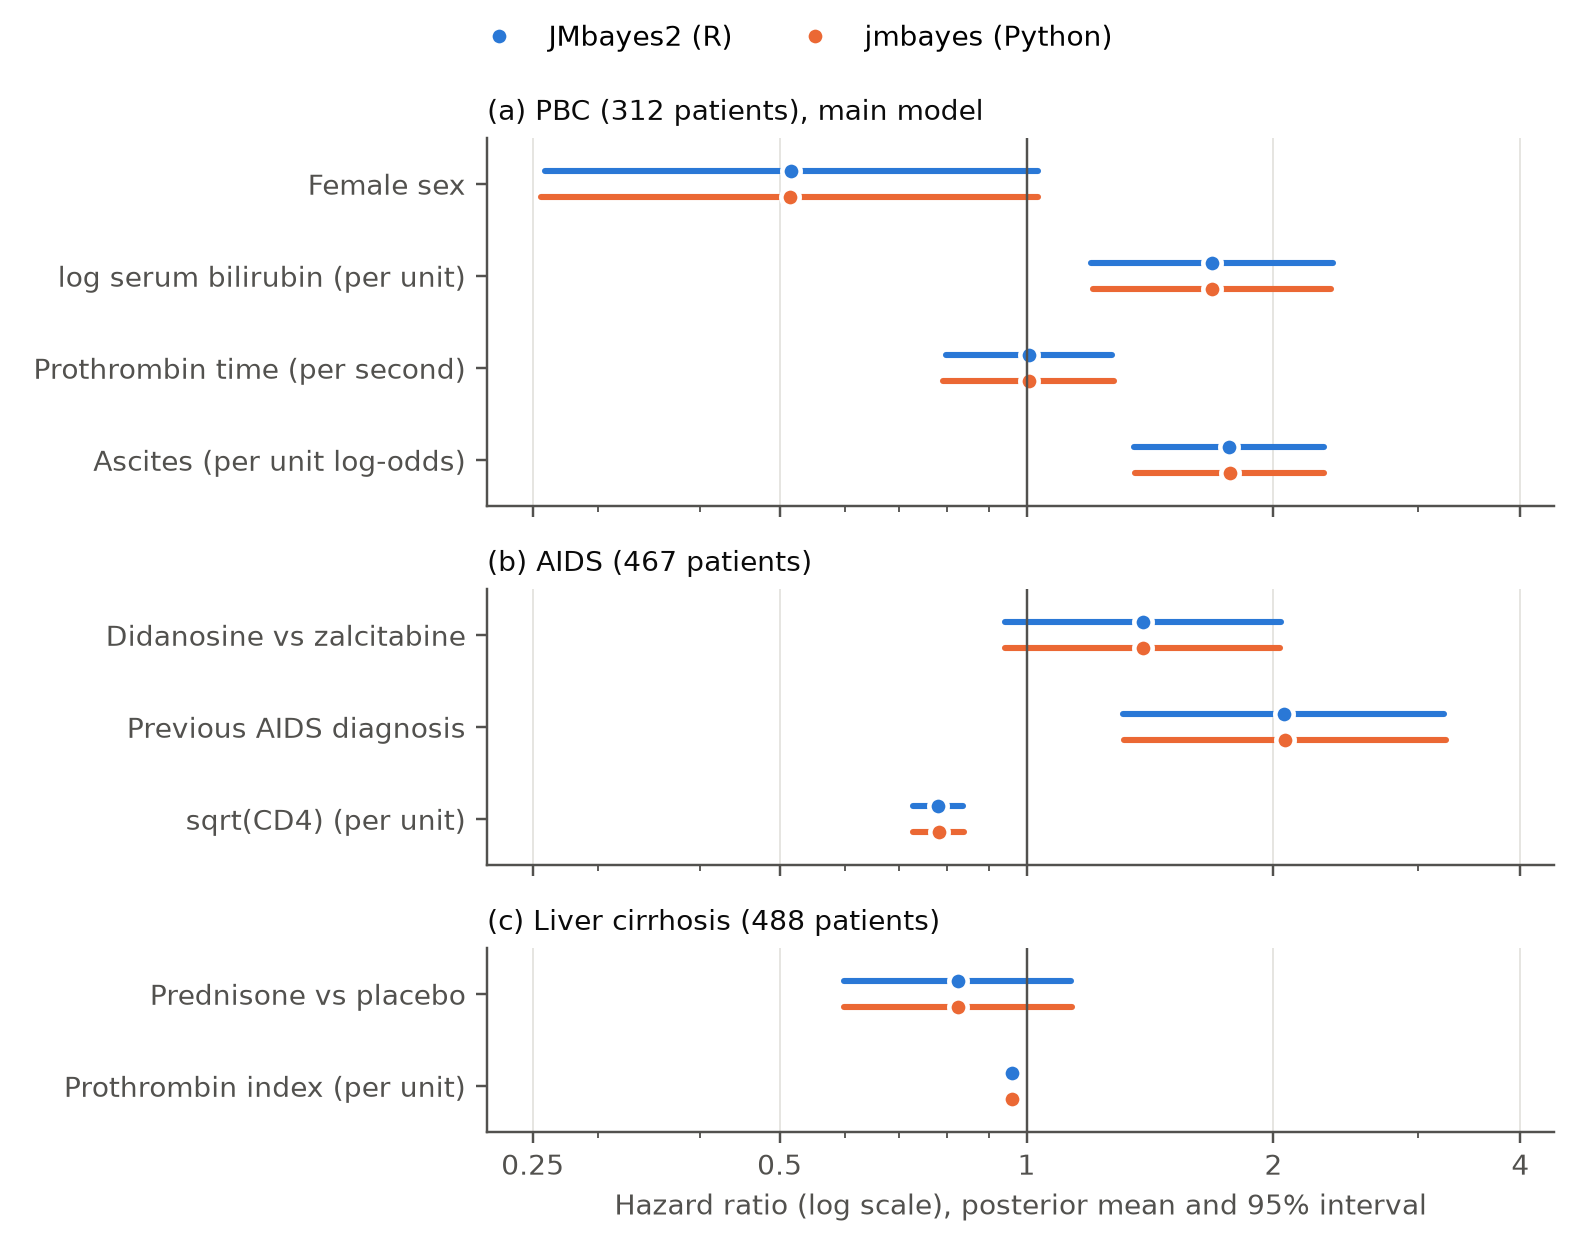
\includegraphics[width=0.85\linewidth]{figures/forest.png}
\caption{Hazard ratios in JMbayes2 and jmbayes on the three data sets: (a) the main PBC
model of this section, (b, c) the two other data sets that ship with JMbayes2
(Section~\ref{sec:other}). Posterior mean and 95\% interval (mean $\pm$ 1.96 posterior SD
of the log hazard ratio), two seeds averaged per program.}
\label{fig:forest}
\end{figure}

\paragraph{Competing risks.} jmbayes also fits cause-specific hazards for competing events,
the model JMbayes2 fits with \texttt{crisk\_setup()} and \texttt{strata()}: each cause has
its own baseline hazard, covariate effects and marker associations, and predictions give
the cumulative incidence of each cause. We fitted death and transplantation in PBC as
competing events, with cause-specific effects of sex and of the current values of log
serum bilirubin and prothrombin time, in both programs (two seeds each, 12 chains of
30,000 iterations). None of the 50 parameters was shown to differ; 36 were shown
equivalent within $\pm 0.2$ posterior SD and 27 within $\pm 0.1$ SD, the rest being
inconclusive at this run length. The largest difference between the programs, 0.065 SD,
was smaller than between two JMbayes2 runs with different seeds (0.18 SD). Hazard ratios
agreed to two decimals; for example, per unit of log bilirubin, 3.27 (JMbayes2) and 3.27
(jmbayes) for death and 3.66 and 3.64 for transplantation. JMbayes2 0.6-5's
\texttt{predict()} fails on this model, so cumulative incidences were checked internally:
summed over causes, they matched one minus the overall survival to within 0.004.

\paragraph{Prediction accuracy.} jmbayes also ports JMbayes2's measures of predictive
accuracy for dynamic predictions: time-dependent ROC curves and AUC, the Brier score
(also integrated over the prediction window), and calibration (ICI, E50, E90 and the
calibration curve), with model-based or inverse-probability-of-censoring weights. Given the
same predicted risks, they reproduced JMbayes2's values to $10^{-10}$ or better in two
prediction windows.

\paragraph{Other markers, strata and late entry.} jmbayes 0.6 adds Poisson, negative
binomial and Student's $t$ markers, stratified baseline hazards and delayed entry (left
truncation), with JMbayes2's densities, priors and quadrature (a 7-point Gauss--Kronrod
rule on $[\text{entry}, T_i]$ under delayed entry). We tested two models as above (two
seeds, 12 chains of 30,000 iterations). In the first, the baseline hazard was stratified by
treatment, entry was set to 20\% of follow-up, and log serum bilirubin and prothrombin
time were Gaussian markers; all 47 parameters were shown equivalent within $\pm 0.1$ SD
(largest difference 0.032 SD). In the second, platelets were negative binomial, rounded
serum bilirubin Poisson and prothrombin time Student's $t$ with 4 degrees of freedom; all
50 parameters were shown equivalent within $\pm 0.1$ SD (largest 0.034 SD). Because
GLMMadaptive's Student's $t$ fit did not converge and \texttt{jm()} centres some priors on
the separate fits, both programs started from R's separate fits in the second model. MCMC
took 1,712~s and 3,907~s in JMbayes2 and 135~s and 173~s in jmbayes.

\paragraph{Further features.} jmbayes 0.7 and 0.8 add the rest of JMbayes2's model options:
beta, gamma, censored normal, beta-binomial and binomial (with trials) markers;
time-varying survival covariates (counting-process rows); interval censoring; recurrent
events with a terminal event and a frailty; competing risks combined with delayed entry and
strata; effects per stratum; all functional forms (velocity, acceleration, area and Delta
with time windows, transformations such as expit and Dexp, interactions with covariates,
and time-varying associations); Weibull, piecewise-constant and natural-spline baseline
hazards; multi-state models; case weights; ridge and horseshoe shrinkage priors; and
marginal fit statistics. We tested each with one model, in both programs, with two seeds
of 8 chains and 15,000 iterations, using the same equivalence test. To check data other
than PBC, we also fitted a model to each of two other data sets that ship with JMbayes2:
CD4 counts and death in 467 HIV patients (\texttt{aids}), and the prothrombin index and
death in 488 patients with liver cirrhosis (\texttt{prothro}).

Table~\ref{tab:ext} gives the results, together with the main model and the competing-risks
model above, so that every model in this paper is judged the same way. No parameter in any
of the 21 further models was shown to differ between the programs. Per parameter, the equivalence tests
(Table~\ref{tab:extdetail} in the appendix) showed all or nearly all parameters equivalent
within $\pm 0.2$ SD in 16 models; in the other five (competing risks with delayed entry and
strata, recurrent events, effects per stratum, the beta-binomial model and the multi-state
model) many were inconclusive, but two runs of the same program differed about
as much as the two programs did, which points to slow mixing at this run length rather
than to a difference. In the beta-binomial model, for example, the random intercepts of
the two markers correlate at 0.98, so their associations with the hazard are nearly
confounded.

Figure~\ref{fig:hrscatter}a compares all 89 hazard ratios of all 23 models in this paper
(each listed in Table~\ref{tab:hrall} in the appendix). MCMC estimates carry Monte Carlo
error, so even two JMbayes2 runs with different seeds do not give identical hazard ratios;
the yardstick is therefore whether jmbayes differs from JMbayes2 more than JMbayes2
differs from itself. It does not (Figure~\ref{fig:hrscatter}b): between single runs, 70\%
of hazard ratios agreed within 1\% for JMbayes2 against itself with another seed, and 74\%
for JMbayes2 against jmbayes (median difference 0.39\% and 0.26\%). The two distributions
coincide, so the differences are the Monte Carlo error that any rerun of JMbayes2 shows. The larger differences are in the
slowly mixing models, where the two programs' own runs also differ, most of all in the
beta-binomial model, whose associations are nearly confounded.

\paragraph{Other data sets.}\label{sec:other} The tests above, like the main comparison, use the PBC data.
To check that agreement does not depend on that data set, we fitted a joint model to each
of the two other data sets that ship with JMbayes2. In the AIDS data (467 patients
randomised to didanosine or zalcitabine), the square root of the CD4 count, with a random
intercept and slope over time, was linked to death, adjusting for drug and a previous AIDS
diagnosis. In the liver cirrhosis data (488 patients randomised to prednisone or placebo),
the prothrombin index was linked to death, adjusting for treatment. In both, all 22
parameters were shown equivalent within $\pm 0.2$ SD (18 and 19 within $\pm 0.1$ SD), and
the hazard ratios agreed to the third decimal (Figure~\ref{fig:forest}b and c, drawn
and computed exactly as for PBC in panel a); for example, 1.39
in both programs for didanosine and 0.83 in both for prednisone.

\begin{figure}[t]
\centering
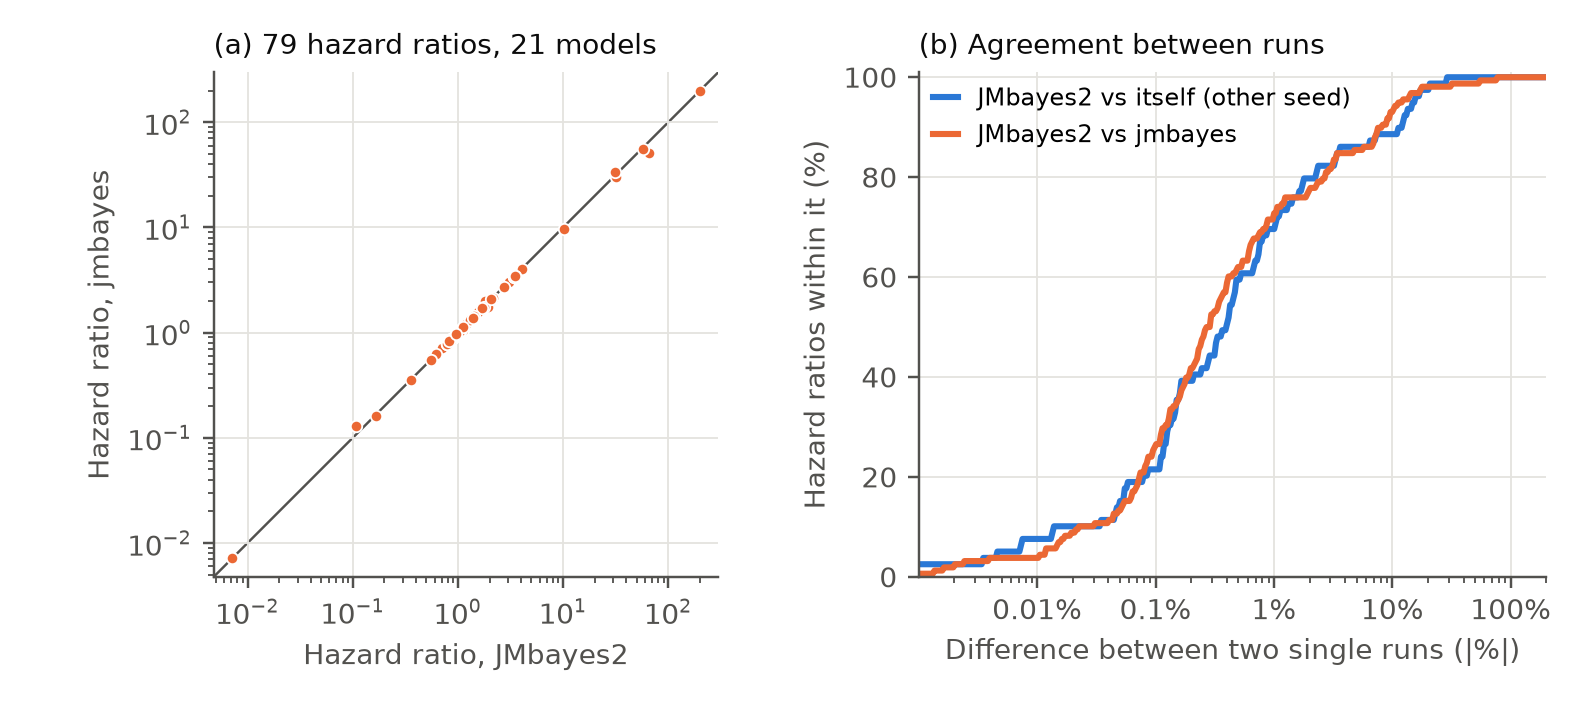
\includegraphics[width=\linewidth]{figures/hr_scatter.png}
\caption{(a) All hazard ratios of all 23 models, jmbayes against
JMbayes2 (posterior means, two seeds averaged; the line is equality). (b) Agreement between
single runs: the share of hazard ratios (y) whose relative difference is at most x, for
JMbayes2 against itself run with another seed (blue) and JMbayes2 against jmbayes
(orange). The curves coincide: jmbayes differs from JMbayes2 no more than JMbayes2 differs
from itself.}
\label{fig:hrscatter}
\end{figure}
The comparisons also found an error in jmbayes: for markers whose density is a difference of
large log-gamma terms (beta-binomial, negative binomial, beta and gamma), 32-bit rounding
exceeded the signal at large dispersions, and the beta-binomial dispersion drifted
upwards. These densities are now computed in 64-bit precision, and the affected
comparisons were rerun. On the AIDS data, statsmodels' default optimiser stopped at a poor
optimum of the separate linear mixed model (its REML log-likelihood 739 units below the
maximum), which moved the priors centred on that fit; jmbayes now also tries Powell's
method and keeps the better fit, and the results in Table~\ref{tab:ext} use this. These runs shared the machine with each other, so we do not report
their timings; Section~\ref{sec:bench} measures speed.

\begin{longtable}{lrrrr}
\caption{jmbayes against JMbayes2 for every model in this paper, judged the same way: two runs per program with different seeds (12 chains of 30,000 iterations for the first four models, 8 of 15,000 for the rest). Shown to differ: parameters whose difference is shown to exceed 0.2 posterior SD (two one-sided tests at 5\%). Difference: between a JMbayes2 run and a jmbayes run, per parameter, in units of its posterior SD (median and largest over the parameters). Equivalence counts per model are in Table~\ref{tab:extdetail}; Section~\ref{sec:multi} repeats the comparison with 30 runs per program.}\label{tab:ext}\\
\toprule & & Shown to & \multicolumn{2}{c}{Difference (posterior SDs)} \\
\cmidrule(lr){4-5}
Model & Parameters & differ & Median & Largest \\ \midrule \endfirsthead
\toprule & & Shown to & \multicolumn{2}{c}{Difference (posterior SDs)} \\
\cmidrule(lr){4-5}
Model & Parameters & differ & Median & Largest \\ \midrule \endhead
\bottomrule \endlastfoot
Main model (PBC, 3 markers) & 50 & 0 & 0.020 & 0.096 \\
Competing risks (PBC) & 50 & 0 & 0.021 & 0.068 \\
Strata + late entry & 47 & 0 & 0.015 & 0.033 \\
NB, Poisson, Student's $t$ & 50 & 0 & 0.012 & 0.037 \\
Time-varying covariate & 23 & 0 & 0.021 & 0.037 \\
Interval censoring & 22 & 0 & 0.024 & 0.080 \\
Competing risks + entry + strata & 60 & 0 & 0.111 & 0.231 \\
Effects per stratum & 50 & 0 & 0.044 & 0.180 \\
Recurrent events & 38 & 0 & 0.103 & 0.154 \\
Gamma, beta, cens.\ normal & 50 & 0 & 0.019 & 0.063 \\
Binomial (trials), beta-binomial & 25 & 0 & 0.130 & 0.500 \\
Velocity, area & 27 & 0 & 0.045 & 0.115 \\
expit, Dexp, acceleration & 27 & 0 & 0.055 & 0.120 \\
Value by sex, Delta & 27 & 0 & 0.034 & 0.071 \\
Time-varying association & 26 & 0 & 0.022 & 0.089 \\
Weibull baseline & 12 & 0 & 0.010 & 0.122 \\
Piecewise-constant baseline & 20 & 0 & 0.014 & 0.041 \\
Natural-spline baseline & 21 & 0 & 0.011 & 0.038 \\
Multi-state & 18 & 0 & 0.028 & 0.140 \\
Case weights & 22 & 0 & 0.014 & 0.057 \\
Shrinkage priors & 39 & 0 & 0.019 & 0.103 \\
AIDS data & 22 & 0 & 0.027 & 0.068 \\
Prothrombin data & 22 & 0 & 0.021 & 0.079 \\
\end{longtable}


\section{Speed and memory}\label{sec:bench}

\paragraph{Setup.} To vary the cohort size, the PBC data were copied 1, 2, 5 and 10 times
with new patient identifiers (312 to 3,120 patients). We fitted the same model with 3
chains (burn-in 500, thinning 5) at 3,500 iterations (JMbayes2's default) and, for 1,560
and 3,120 patients, up to 90,000 iterations. Each run was a separate process, run one at a
time. Peak RAM is the resident memory of the whole process tree, sampled every 0.2~s, which
includes JMbayes2's worker processes (one per chain). MCMC time excludes the initial
separate model fits, which both programs need. JMbayes2 runs its chains in parallel on the
CPU; jmbayes ran on the GPU in 32-bit precision. All runs used one machine: Intel Core
i9-12900K (x86-64; 16 cores, 8 performance and 8 efficiency, 24 threads), 64~GB RAM, NVIDIA
GeForce RTX 3090 (24~GB), Windows 11, R 4.6.2 with JMbayes2 0.6-5, Python 3.11 with PyTorch
2.6 (CUDA 12.4).

\paragraph{Results.} Table~\ref{tab:bench} and Figure~\ref{fig:bench} show the results.
jmbayes was 3.3$\times$ faster on 312 patients and 8.0--8.6$\times$ faster on 1,560--3,120
patients at the default length, and 9.7--10.5$\times$ on long runs: at 90,000 iterations
for 3,120 patients, JMbayes2 took 104 minutes and 37.8~GB of RAM, and jmbayes 11 minutes
and 1.4~GB. Ten times more patients increased jmbayes's MCMC time 1.4-fold and JMbayes2's
3.7-fold. jmbayes's RAM stayed at 1.3--1.4~GB and its GPU memory below 0.2~GB in every
run, up to 90,000 iterations, while JMbayes2's memory grew with both patients and
iterations.

The speed comes from the GPU. Run on the CPU alone, jmbayes was about as fast as JMbayes2
on small cohorts and slower on large ones (445~s vs 202~s for 3,120 patients at 3,500
iterations), but used less than half the memory (0.6--0.7~GB).

\begin{table}[t]
\centering
\caption{MCMC time and peak RAM. jmbayes on the GPU in 32-bit precision; JMbayes2 on the
CPU. Dashes: not run.}
\label{tab:bench}
\vspace{4pt}
\begin{tabular}{rrrrrrr}
\toprule
& & \multicolumn{2}{c}{JMbayes2} & \multicolumn{2}{c}{jmbayes} & \\
\cmidrule(lr){3-4}\cmidrule(lr){5-6}
Patients & Iterations & Time & RAM & Time & RAM & Speed-up \\
\midrule
312   & 3,500  & 55 s    & 1.28 GB & 17 s  & 1.28 GB & 3.3$\times$ \\
624   & 3,500  & 87 s    & 1.45 GB & 17 s  & 1.28 GB & 5.0$\times$ \\
1,560 & 3,500  & 157 s   & 1.95 GB & 20 s  & 1.29 GB & 8.0$\times$ \\
3,120 & 3,500  & 202 s   & 2.41 GB & 24 s  & 1.31 GB & 8.6$\times$ \\
1,560 & 7,000  & 237 s   & 2.34 GB & 41 s  & 1.29 GB & 5.8$\times$ \\
1,560 & 14,000 & 716 s   & 3.36 GB & 82 s  & 1.30 GB & 8.8$\times$ \\
1,560 & 28,000 & 1,046 s & 6.25 GB & 164 s & 1.31 GB & 6.4$\times$ \\
3,120 & 7,000  & 450 s   & 3.44 GB & 48 s  & 1.31 GB & 9.4$\times$ \\
3,120 & 14,000 & 521 s   & 6.15 GB & 96 s  & 1.32 GB & 5.4$\times$ \\
3,120 & 28,000 & 2,056 s & 12.0 GB & 196 s & 1.33 GB & 10.5$\times$ \\
3,120 & 60,000 & 5,893 s$^a$ & 25.2 GB & 429 s & 1.39 GB & \\
1,560 & 90,000 & --      & --      & 529 s & 1.36 GB & \\
3,120 & 90,000 & 6,266 s & 37.8 GB & 643 s & 1.38 GB & 9.7$\times$ \\
\bottomrule
\end{tabular}

\smallskip
\parbox{0.9\linewidth}{\footnotesize $^a$ This run overlapped with other work on the machine. JMbayes2's time per iteration was 98~ms, against 70--73~ms at 28,000 and 90,000 iterations, so this time is likely inflated and no speed-up is given.}
\end{table}

\begin{figure}[t]
\centering
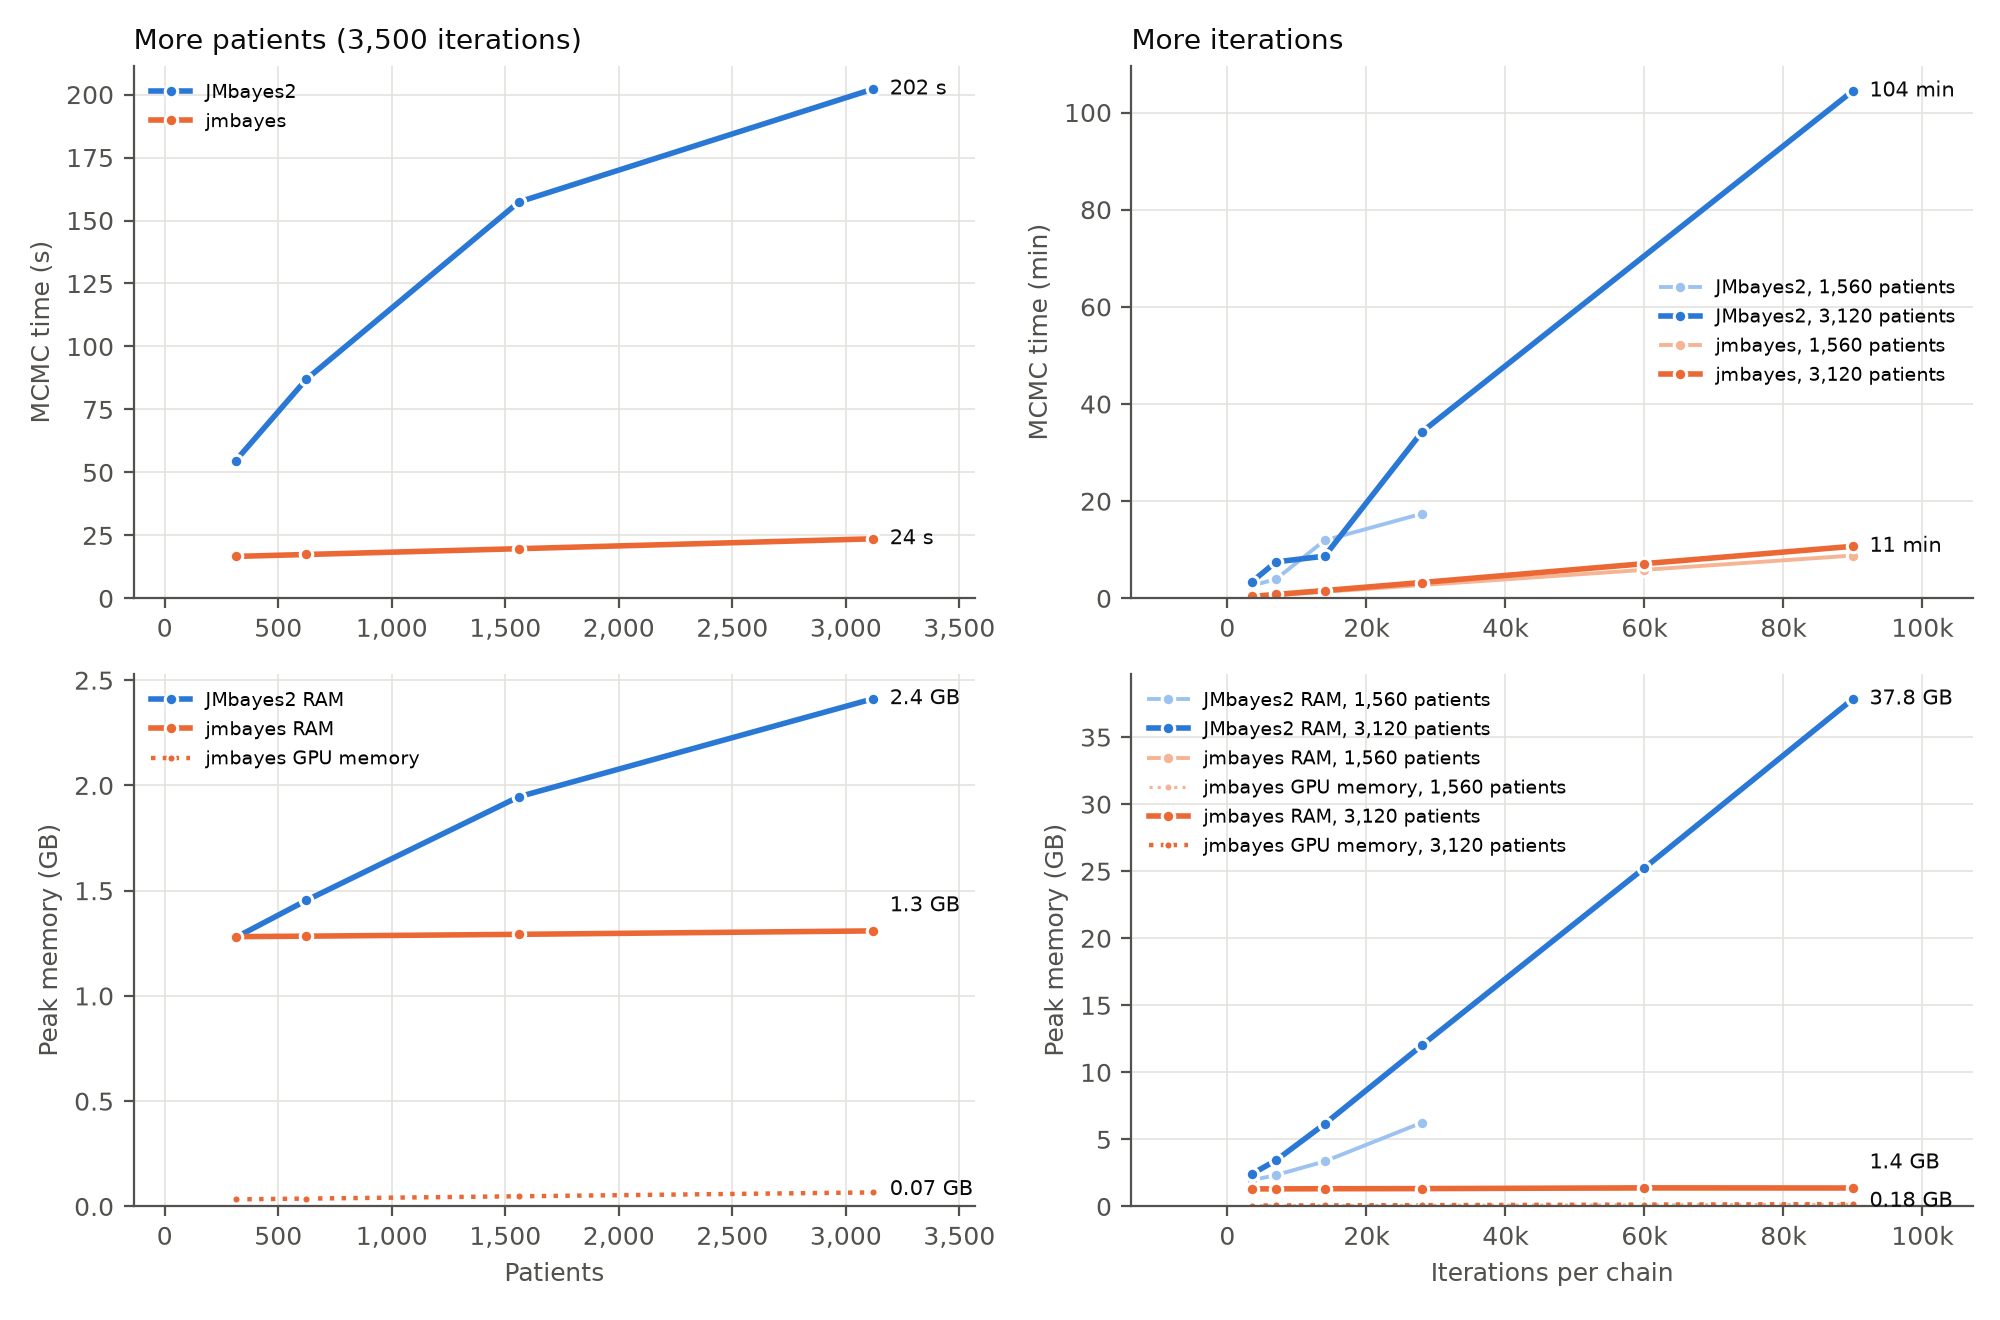
\includegraphics[width=\linewidth]{figures/benchmarks.png}
\caption{MCMC time (top) and peak memory (bottom) as the number of patients (left, 3,500
iterations) and the number of iterations (right; light lines 1,560 patients, dark lines
3,120) grow. Dotted: jmbayes GPU memory.}
\label{fig:bench}
\end{figure}

\section{Limitations}

Each benchmark setting was run once, so single timings carry noise; for example, JMbayes2
took less time for 3,120 patients at 14,000 iterations than for 1,560, and its run at
60,000 iterations overlapped with other work (Table~\ref{tab:bench}). Larger cohorts were
made by copying one data set, which tests scaling but not new data. Equivalence was tested
in depth on one model and data set; three further models (splines, slope and area
associations, fixed effects without random effects) agreed in smaller tests, and
each later feature (marker families, strata, delayed entry, competing risks, interval
censoring, recurrent events, functional forms, baseline hazards, multi-state models, case
weights and shrinkage priors) was tested on one or two models, mostly of the same data.
The speed-up needs a GPU that PyTorch drives through its CUDA interface: NVIDIA
(tested here) or AMD with ROCm (not tested). Apple and Intel GPUs are not supported
yet; there jmbayes runs on the CPU. On a CPU it is about as fast as JMbayes2, because it
runs all chains in one process, which uses only the data parallelism. Combining both
levels of Section~\ref{sec:design}, with groups of chains in separate processes (MIMD, as
JMbayes2) and patients batched within each (SIMD), should make the CPU version faster too;
we leave this to future work. jmbayes covers JMbayes2's model options, with three
exceptions: survival covariates that are functions of the time variable (an interaction
in the association gives the same time-varying effects), interval censoring or recurrent
events combined with delayed entry or competing risks, and dynamic predictions for
recurrent-event models. These stop with an error rather than fitting a different model.

\section{Availability}

jmbayes 0.8.0 is available from PyPI (\texttt{pip install jmbayes}) and at
\url{https://github.com/neuratom/jmbayes} under the GPL-3.0 licence, like JMbayes2. The
repository contains the scripts and results for every number in this paper, including the
full equivalence report. jmbayes is an independent reimplementation and is not affiliated
with or endorsed by the authors of JMbayes2, whose work it builds on.

\begin{thebibliography}{99}

\bibitem{jmbayes2}
D.~Rizopoulos, G.~Papageorgiou and P.~Miranda Afonso.
\newblock JMbayes2: Extended joint models for longitudinal and time-to-event data.
\newblock R package, \url{https://github.com/drizopoulos/JMbayes2}.

\bibitem{rizopoulos2012}
D.~Rizopoulos.
\newblock \emph{Joint Models for Longitudinal and Time-to-Event Data: With Applications
in R}.
\newblock Chapman \& Hall/CRC, 2012.

\bibitem{tsiatis2004}
A.~A. Tsiatis and M.~Davidian.
\newblock Joint modeling of longitudinal and time-to-event data: an overview.
\newblock \emph{Statistica Sinica}, 14:809--834, 2004.

\bibitem{pytorch}
A.~Paszke et al.
\newblock PyTorch: an imperative style, high-performance deep learning library.
\newblock In \emph{Advances in Neural Information Processing Systems 32}, 2019.

\bibitem{spiegelhalter2002}
D.~J. Spiegelhalter, N.~G. Best, B.~P. Carlin and A.~van~der Linde.
\newblock Bayesian measures of model complexity and fit.
\newblock \emph{Journal of the Royal Statistical Society: Series B}, 64(4):583--639, 2002.

\bibitem{watanabe2010}
S.~Watanabe.
\newblock Asymptotic equivalence of Bayes cross validation and widely applicable
information criterion in singular learning theory.
\newblock \emph{Journal of Machine Learning Research}, 11:3571--3594, 2010.

\bibitem{geisser1979}
S.~Geisser and W.~F. Eddy.
\newblock A predictive approach to model selection.
\newblock \emph{Journal of the American Statistical Association}, 74(365):153--160, 1979.

\bibitem{welford1962}
B.~P. Welford.
\newblock Note on a method for calculating corrected sums of squares and products.
\newblock \emph{Technometrics}, 4(3):419--420, 1962.

\bibitem{chan1983}
T.~F. Chan, G.~H. Golub and R.~J. LeVeque.
\newblock Algorithms for computing the sample variance: analysis and recommendations.
\newblock \emph{The American Statistician}, 37(3):242--247, 1983.

\bibitem{vehtari2017}
A.~Vehtari, A.~Gelman and J.~Gabry.
\newblock Practical Bayesian model evaluation using leave-one-out cross-validation and
WAIC.
\newblock \emph{Statistics and Computing}, 27:1413--1432, 2017.

\bibitem{murtaugh1994}
P.~A. Murtaugh, E.~R. Dickson, G.~M. Van~Dam, M.~Malinchoc, P.~M. Grambsch, A.~L.
Langworthy and C.~H. Gips.
\newblock Primary biliary cirrhosis: prediction of short-term survival based on repeated
patient visits.
\newblock \emph{Hepatology}, 20(1):126--134, 1994.

\bibitem{schuirmann1987}
D.~J. Schuirmann.
\newblock A comparison of the two one-sided tests procedure and the power approach for
assessing the equivalence of average bioavailability.
\newblock \emph{Journal of Pharmacokinetics and Biopharmaceutics}, 15(6):657--680, 1987.

\bibitem{gelman1992}
A.~Gelman and D.~B. Rubin.
\newblock Inference from iterative simulation using multiple sequences.
\newblock \emph{Statistical Science}, 7(4):457--472, 1992.

\end{thebibliography}

\appendix
\section{Equivalence tests per model}

\begingroup\small\setlength{\tabcolsep}{4pt}
\begin{longtable}{lrrrrrrr}
\caption{Equivalence tests per model (the runs of Table~\ref{tab:ext}). Each parameter is either shown equivalent (within $\pm 0.2$ posterior SD; the $\pm 0.1$ count is a subset), shown to differ (by more than 0.2 SD), or inconclusive: two runs per program are too few to separate a difference below 0.2 SD from Monte Carlo error, which happens where the chains mix slowly. No parameter was shown to differ. Largest difference: between the programs (R vs Python, seeds averaged) and between the two JMbayes2 runs of the same model (R vs R).}\label{tab:extdetail}\\
\toprule & & \multicolumn{2}{c}{Equivalent} & Incon- & & \multicolumn{2}{c}{Largest diff.} \\
\cmidrule(lr){3-4}\cmidrule(lr){7-8}
Model & Param. & $\pm 0.1$ & $\pm 0.2$ & clusive & Differ & R--Py & R--R \\ \midrule \endfirsthead
\toprule & & \multicolumn{2}{c}{Equivalent} & Incon- & & \multicolumn{2}{c}{Largest diff.} \\
\cmidrule(lr){3-4}\cmidrule(lr){7-8}
Model & Param. & $\pm 0.1$ & $\pm 0.2$ & clusive & Differ & R--Py & R--R \\ \midrule \endhead
\bottomrule \endlastfoot
Main model (PBC, 3 markers) & 50 & 43 & 50 & 0 & 0 & 0.042 & 0.141 \\
Competing risks (PBC) & 50 & 27 & 36 & 14 & 0 & 0.065 & 0.181 \\
Strata + late entry & 47 & 47 & 47 & 0 & 0 & 0.032 & 0.086 \\
NB, Poisson, Student's $t$ & 50 & 50 & 50 & 0 & 0 & 0.034 & 0.062 \\
Time-varying covariate & 23 & 23 & 23 & 0 & 0 & 0.026 & 0.051 \\
Interval censoring & 22 & 17 & 22 & 0 & 0 & 0.077 & 0.113 \\
Competing risks + entry + strata & 60 & 12 & 21 & 39 & 0 & 0.231 & 0.269 \\
Effects per stratum & 50 & 26 & 34 & 16 & 0 & 0.056 & 0.121 \\
Recurrent events & 38 & 12 & 23 & 15 & 0 & 0.154 & 0.107 \\
Gamma, beta, cens.\ normal & 50 & 46 & 50 & 0 & 0 & 0.038 & 0.108 \\
Binomial (trials), beta-binomial & 25 & 6 & 7 & 18 & 0 & 0.244 & 0.139 \\
Velocity, area & 27 & 9 & 25 & 2 & 0 & 0.115 & 0.219 \\
expit, Dexp, acceleration & 27 & 20 & 25 & 2 & 0 & 0.120 & 0.060 \\
Value by sex, Delta & 27 & 22 & 27 & 0 & 0 & 0.071 & 0.041 \\
Time-varying association & 26 & 25 & 26 & 0 & 0 & 0.045 & 0.087 \\
Weibull baseline & 12 & 10 & 12 & 0 & 0 & 0.025 & 0.114 \\
Piecewise-constant baseline & 20 & 20 & 20 & 0 & 0 & 0.031 & 0.046 \\
Natural-spline baseline & 21 & 21 & 21 & 0 & 0 & 0.023 & 0.056 \\
Multi-state & 18 & 12 & 12 & 6 & 0 & 0.115 & 0.316 \\
Case weights & 22 & 22 & 22 & 0 & 0 & 0.057 & 0.039 \\
Shrinkage priors & 39 & 26 & 37 & 2 & 0 & 0.045 & 0.273 \\
AIDS data & 22 & 18 & 22 & 0 & 0 & 0.064 & 0.032 \\
Prothrombin data & 22 & 19 & 22 & 0 & 0 & 0.041 & 0.129 \\
\end{longtable}
\endgroup


\section{Hazard ratios of every model}

\begingroup\small\setlength{\tabcolsep}{4pt}
\begin{longtable}{llrr}
\caption{Hazard ratios (posterior means, two seeds averaged) in JMbayes2 and jmbayes; up to 4 per model (all are in the repository).}\label{tab:hrall}\\
\toprule Model & Term & JMbayes2 & jmbayes \\ \midrule \endfirsthead
\toprule Model & Term & JMbayes2 & jmbayes \\ \midrule \endhead
\bottomrule \endlastfoot
Main model (PBC, 3 markers) & \texttt{sexfemale} & 0.517 & 0.515 \\
 & \texttt{value(log(serBilir))} & 1.683 & 1.681 \\
 & \texttt{value(prothrombin)} & 1.008 & 1.006 \\
 & \texttt{value(ascites)} & 1.767 & 1.769 \\
\addlinespace
Competing risks (PBC) & \texttt{sexfemale [transplanted]} & 2.169 & 2.140 \\
 & \texttt{sexfemale [dead]} & 0.702 & 0.703 \\
 & \texttt{value(log(serBilir)) [transplan\ldots} & 3.658 & 3.644 \\
 & \texttt{value(log(serBilir)) [dead]} & 3.271 & 3.269 \\
\addlinespace
Strata + late entry & \texttt{sexfemale} & 0.811 & 0.809 \\
 & \texttt{value(log(serBilir))} & 2.972 & 2.965 \\
 & \texttt{value(prothrombin)} & 1.203 & 1.203 \\
\addlinespace
NB, Poisson, Student's $t$ & \texttt{sexfemale} & 0.909 & 0.907 \\
 & \texttt{value(platelets)} & 0.580 & 0.584 \\
 & \texttt{value(bili\_count)} & 3.607 & 3.603 \\
 & \texttt{value(prothrombin)} & 1.444 & 1.448 \\
\addlinespace
Time-varying covariate & \texttt{sexfemale} & 0.675 & 0.676 \\
 & \texttt{edema\_tv} & 3.248 & 3.242 \\
 & \texttt{value(log(serBilir))} & 2.892 & 2.895 \\
\addlinespace
Interval censoring & \texttt{sexfemale} & 0.896 & 0.896 \\
 & \texttt{value(log(serBilir))} & 3.521 & 3.528 \\
\addlinespace
Competing risks + entry + strata & \texttt{sexfemale [transplanted]} & 2.071 & 1.999 \\
 & \texttt{sexfemale [dead]} & 0.750 & 0.755 \\
 & \texttt{value(log(serBilir)) [transplan\ldots} & 3.546 & 3.464 \\
 & \texttt{value(log(serBilir)) [dead]} & 3.100 & 3.098 \\
\addlinespace
Effects per stratum & \texttt{sexfemale [placebo]} & 0.777 & 0.781 \\
 & \texttt{sexfemale [D-penicil]} & 0.865 & 0.876 \\
 & \texttt{value(log(serBilir)) [placebo]} & 3.083 & 3.092 \\
 & \texttt{value(log(serBilir)) [D-penicil]} & 3.407 & 3.408 \\
\addlinespace
Recurrent events & \texttt{group [R]} & 1.615 & 1.616 \\
 & \texttt{group [T1]} & 1.571 & 1.566 \\
 & \texttt{age [R]} & 1.052 & 1.052 \\
 & \texttt{age [T1]} & 1.049 & 1.048 \\
\addlinespace
Gamma, beta, cens.\ normal & \texttt{sexfemale} & 0.705 & 0.707 \\
 & \texttt{value(serBilir)} & 3.058 & 3.052 \\
 & \texttt{value(alb\_p)} & 0.007 & 0.007 \\
 & \texttt{value(lalk)} & 0.622 & 0.623 \\
\addlinespace
Binomial (trials), beta-binomial & \texttt{sexfemale} & 1.105 & 1.059 \\
 & \texttt{value(count2)} & 0.107 & 0.128 \\
 & \texttt{value(count3)} & 65.843 & 50.888 \\
\addlinespace
Velocity, area & \texttt{sexfemale} & 0.836 & 0.835 \\
 & \texttt{value(log(serBilir))} & 1.801 & 1.985 \\
 & \texttt{velocity(log(serBilir), eps = 0\ldots} & 32.075 & 30.115 \\
 & \texttt{area(log(serBilir), time\_windo\ldots} & 1.920 & 1.744 \\
\addlinespace
expit, Dexp, acceleration & \texttt{sexfemale} & 0.779 & 0.774 \\
 & \texttt{vexpit(value(log(serBilir)))} & 198.969 & 195.992 \\
 & \texttt{acceleration(log(serBilir))} & 31.266 & 33.295 \\
 & \texttt{vexp(value(log(serBilir))):slop\ldots} & 1.330 & 1.331 \\
\addlinespace
Value by sex, Delta & \texttt{sexfemale} & 0.549 & 0.544 \\
 & \texttt{Delta(log(serBilir), time\_wind\ldots} & 10.120 & 9.674 \\
 & \texttt{value(log(serBilir)):sexmale} & 2.735 & 2.738 \\
 & \texttt{value(log(serBilir)):sexfemale} & 3.389 & 3.404 \\
\addlinespace
Time-varying association & \texttt{sexfemale} & 0.862 & 0.863 \\
 & \texttt{value(log(serBilir))} & 4.020 & 4.022 \\
 & \texttt{value(log(serBilir)):ns(year, k\ldots} & 0.799 & 0.800 \\
 & \texttt{value(log(serBilir)):ns(year, k\ldots} & 0.824 & 0.827 \\
\addlinespace
Weibull baseline & \texttt{sexfemale} & 0.831 & 0.832 \\
 & \texttt{value(log(serBilir))} & 3.423 & 3.419 \\
\addlinespace
Piecewise-constant baseline & \texttt{sexfemale} & 0.852 & 0.852 \\
 & \texttt{value(log(serBilir))} & 3.485 & 3.484 \\
\addlinespace
Natural-spline baseline & \texttt{sexfemale} & 0.880 & 0.873 \\
 & \texttt{value(log(serBilir))} & 3.392 & 3.387 \\
\addlinespace
Multi-state & \texttt{X [1]} & 1.563 & 1.563 \\
 & \texttt{X [2]} & 0.784 & 0.784 \\
 & \texttt{X [3]} & 1.770 & 1.770 \\
 & \texttt{value(y) [1]} & 1.704 & 1.704 \\
\addlinespace
Case weights & \texttt{sexfemale} & 0.853 & 0.854 \\
 & \texttt{value(log(serBilir))} & 3.484 & 3.485 \\
\addlinespace
Shrinkage priors & \texttt{sexfemale} & 1.041 & 1.038 \\
 & \texttt{age} & 1.039 & 1.039 \\
 & \texttt{drugD-penicil} & 0.954 & 0.950 \\
 & \texttt{value(log(serBilir))} & 1.423 & 1.452 \\
\addlinespace
AIDS data & \texttt{drugddI} & 1.386 & 1.386 \\
 & \texttt{prevOIAIDS} & 2.060 & 2.065 \\
 & \texttt{value(CD4)} & 0.780 & 0.781 \\
\addlinespace
Prothrombin data & \texttt{treatprednisone} & 0.825 & 0.825 \\
 & \texttt{value(pro)} & 0.959 & 0.959 \\
\addlinespace
\end{longtable}
\endgroup


\end{document}
